%
%-----------------------------------
\section{Dysprosium}
\label{sec:dysprosium}
%-----------------------------------
%

The dysprosium nMOT \cite{dreon2017optical} reproduced by Davide Dreon and his research group matches the conditions of our experiment and is thorough detailed in the Dreon PhD thesis \cite{dreon2017designing}, which is help us to improve accuracy as discussed in section \ref{sec:input-outputs}. Moreover, our research group is preparing a experimental setup to cool and trap dysprosium atoms aiming to study dipolar quantum gases.

\begin{table}[ht!]
    \centering
    \begin{tabular}{|c|c|c|}
        \hline
        \textbf{Symbol} & \textbf{Quantity} & \textbf{Value} \\ \hline
        $ \Gamma / 2\pi $ & Natural Linewidth & $ 136\ kHz $ \\
        $ \lambda $ & Resonant wavelength & $ 626\ nm $ \\
        $ J_{gnd} $ & Ground state angular momentum & $ 8 $ \\
        $ g_{gnd} $ & Ground state Landé factor & $ 1.24 $ \\
        $ J_{exc} $ & Excited state angular momentum & $ 9 $ \\
        $ g_{exc} $ & Excited state Landé factor & $ 1.29 $ \\
        $ m $ & Mass & $ 164\ u $ \\
        \hline
    \end{tabular}
    \caption{Eletronic transition parameters of the dysprosium nMOT reproduced by \cite{dreon2017designing}.}
    \label{tab:electronic-transition-Dy-Dreon}
\end{table}

The involved electronic transition presented in Table \ref{tab:electronic-transition-Dy-Dreon} yields a narrowness of $ \eta =  43.8 $ that is enough to reach the power-broadened regime for large laser detunings. This transition is more complicated than the one present in Chapter \ref{ch:Monte-Carlo-simulation} since it has 36 possible states in the presence of a magnetic field. However, in the power-broadened regime, the dysprosium atoms gather in a region with a large and negative magnetic field, which leads to a large and positive Zeeman shift so that an efficient optical pumping populates the absolute ground state $ \ket{J = 8, m_J = -8} $. This spin-polarization phenomenon was observed experimentally for nMOTs with lanthanide atoms \cite{lu2011strongly,aikawa2012bose} and also for the Dreon experiment. Therefore, due to selection rules (see Appendix \ref{ap:selection-rules}), we can simplify the transitions to a four-level system as illustrated in Figure \ref{fig:Dy-Dreon-electronic-transitions} and then apply our model under the three independent two-level systems assumption.

\begin{figure}[!ht]
    \centering
    \caption{Electronic transitions of the dysprosium nMOT}
    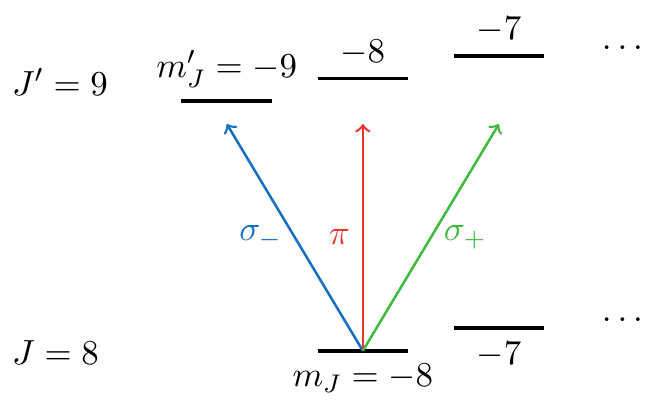
\includegraphics[width=0.5\textwidth]{USPSC-img/Dy-Dreon-transitions.png}
    \vspace{5px}
    \legend{Electronic transitions of dysprosium atoms in a nMOT under the spin-polarization phenomenon. Such phenomenon populates the absolute ground state $ \ket{J = 8, m_J = -8} $. Hence, due to selection rules (see appendix \ref{ap:selection-rules}), we can simplify the transitions to a four-level system $ \ket{J = 8, m_J = 8} \longrightarrow \ket{J' = 9, m_J' = -7, -8, -9} $. \\ Source: \cite{dreon2017optical}}
    \label{fig:Dy-Dreon-electronic-transitions}
\end{figure}

The arrangement of the lasers is not the usual one introduced in Section \ref{eq:three-dimensional-case}, where we have a pair of counter-propagating laser beams in the gravity direction. In the Dreon setup, there are two pairs of counter-propagating laser beams forming an angle of 45 degrees with the gravity direction, as illustrated in Figure \ref{fig:Dreon-setup}. All laser beams have the same saturation parameter of $ s = 0.65 $ and waist of $ w = 2cm $ Moreover, the strong magnetic field axis is perpendicular to the gravity direction. This setup was designed to decrease the MOT force in the gravity direction and then guarantee that the atoms fall below the magnetic field origin. The parameters of the laser arrangement and the magnetic field profile are presented in Tables

\begin{figure}[!ht]
    \centering
    \caption{nMOT setup of the Dreon experiment}
    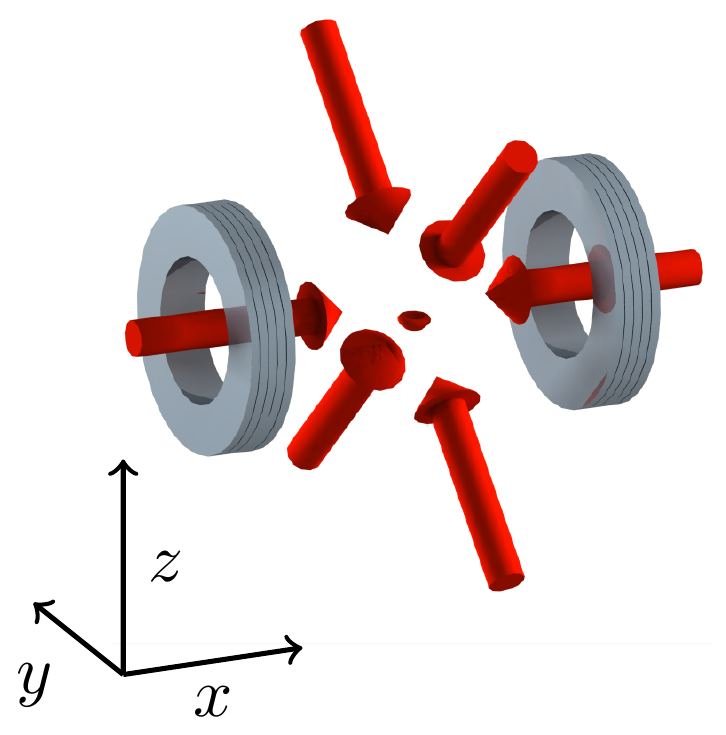
\includegraphics[width=0.35\textwidth]{USPSC-img/Dreon-setup.png}
    \legend{Laser beam arrangement and Helmholtz coils of the Dreon nMOT. \\ Source: author}
    \label{fig:Dreon-setup}
    \vspace{-5px}
\end{figure}

\begin{table}[ht!]
    \centering
    \begin{tabular}{|c|c|}
        \hline
        \textbf{Wave vector (arb. unit.)} & \textbf{Polarization} \\ \hline
        $ (1, 0, 0) $ & $ (0, 1, 0) $ \\
        $ (-1, 0, 0) $ & $ (0, 1, 0) $ \\
        $ (0, 1, 1) $ & $ (1, 0, 0) $ \\
        $ (0, -1, 1) $ & $ (1, 0, 0) $ \\
        $ (0, 1, -1) $ & $ (1, 0, 0) $ \\
        $ (0, -1, -1) $ & $ (1, 0, 0) $ \\
        \hline
    \end{tabular}
    \caption{Wave vector direction $ (x, y, z) $ and polarization $ (\sigma_+, \sigma_-, \pi) $ in the laboratory frame (see Section \ref{sec:magnetic-field-frame}) of the Dreon nMOT.}
    \label{tab:Dreon-laser-beams}
\end{table}

\begin{table}[ht!]
    \centering
    \begin{tabular}{|c|c|c|}
        \hline
        \textbf{Symbol} & \textbf{Quantity} & \textbf{Value} \\ \hline
        $ B_0 $ & Axial gradient & $ 1.71 G $ \\
        $ B $ & Magnetic Field & $ B_0(-\hat{x} + \hat{y}/2 + \hat{z} / 2) $ \\
        $ B_{bias} $ & Bias & $ (-0.094 \hat{z})\ G / cm $ \\
        \hline
    \end{tabular}
    \caption{Magnetic field parameters of the Dreon nMOT}
    \label{tab:Dreon-magnetic-field}
\end{table}

%-----------------------------------
\subsection{Atomic cloud profile}
\label{sec:cloud-profile-dysprosium}
%-----------------------------------

The in-situ and simulated atomic cloud profiles are shown in Figures \ref{fig:Dreon-simulated-atomic-cloud-profile} and \ref{fig:Dreon-in-situ-atomic-cloud-profile}. The simulated profile is a heat map of the position distribution presented in equation (\ref{eq:joint-position-distribution}). In both cases, the atomic cloud distribution resembles an ellipsoid whose semimajor axis is perpendicular to the gravity direction. Also, its centre of mass is below the magnetic field's origin. In figure \ref{fig:Dreon-simulated-atomic-cloud-profile}, we can see that the larger the laser detuning, the lower the centre of mass.

\begin{figure}[!ht]
    \centering
    \caption{In-situ and simulated atomic cloud profile of Dreon nMOTs}
    \begin{subfigure}[b]{0.5\linewidth}
        \centering
        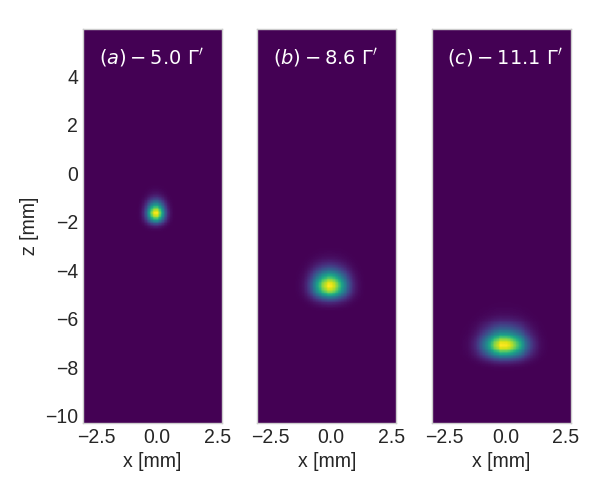
\includegraphics[width=\textwidth]{USPSC-img/dy_dreon_cloud_profile.png}
        \caption{Simulated atomic cloud profile for different laser detunings.}
        \label{fig:Dreon-simulated-atomic-cloud-profile}
    \end{subfigure}
    \hspace{20px}
    \begin{subfigure}[b]{0.3\linewidth}
        \centering
        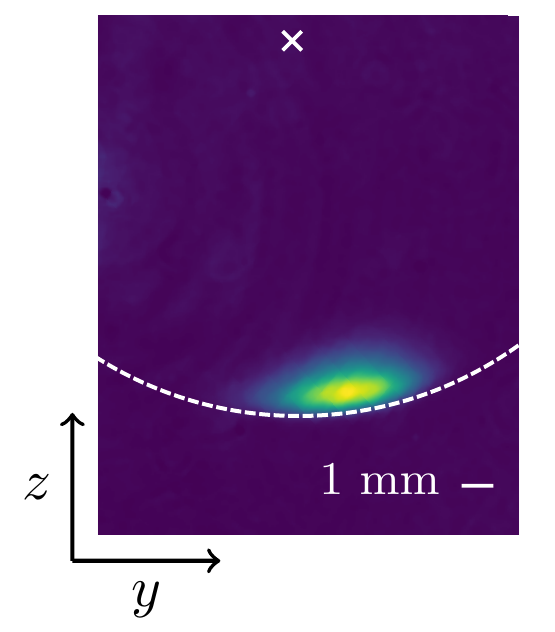
\includegraphics[width=\textwidth]{USPSC-img/in-situ-atomic-cloud-Dreon.png}
        \vspace{18px}
        \caption{In situ atomic cloud profile of the Dreon nMOT}
        \label{fig:Dreon-in-situ-atomic-cloud-profile}
    \end{subfigure}
\end{figure}

From equation (\ref{eq:centre-of-mass-power-broadened-regime}), we expect that the centre of mass\footnote{We are considering only the z component as the centre of mass since all other components is about zero in all cases.} of the atomic cloud is proportional to the laser detuning for large detunings. In fact, the simulated centre of mass given by equation (\ref{eq:simulated-centre-of-mass}) and the experimental measures confirm this linear relation for laser detunings roughly larger than $ 2\pi \times 700\ kHz \simeq 4\Gamma' $, as illustrated in Figure \ref{fig:Dreon-centre-of-mass}. However, the theoretical centre of mass is not as accurate as the simulated one since there is a difference of about $1mm$ between the experimental and theoretical centre of mass, whereas the simulated measures match almost perfectly the experimental measures.

\begin{figure}[!ht]
    \centering
    \caption{Centre of mass of the Dreon nMOT in function of the laser detunings}
    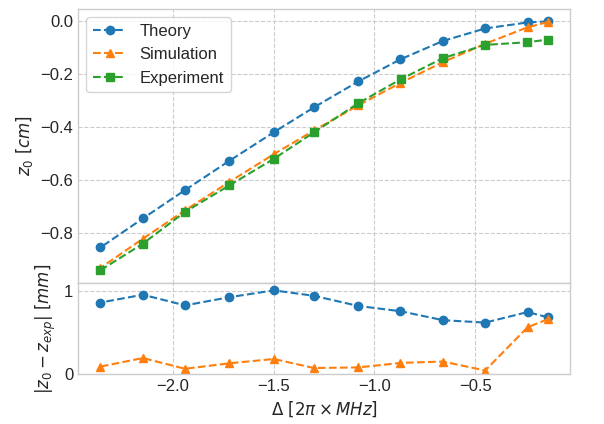
\includegraphics[width=0.7\textwidth]{USPSC-img/dy_centre_of_mass.png}
    \vspace{5px}
    \legend{The gravity direction component of the centre of mass as a function of the laser detuning. The blue spheres, orange triangles, and green squares are, respectively, the theoretical centres of mass from equation (\ref{eq:centre-of-mass-power-broadened-regime}), simulated points, and experimental measures of the Dreon nMOT. \\ Source: author}
    \label{fig:Dreon-centre-of-mass}
\end{figure}

We do not expect an accurate estimative of the cloud size since this quantity is affected by interactions between atoms, which are not taken into account in our model. Indeed, the experimental cloud sized is larger than the simulated ones given by equation (\ref{eq:simulated-cloud-sizes}), as illustrated in Figure \ref{fig:Dreon-cloud-size}. This is expected due to the re-absorption of scattered photons. Nevertheless, we are able to compare the experimental and simulated cloud sizes more clearly by verifying the ratio between two cloud size components, as illustrated in Figure \ref{fig:Dreon-cloud-size-ratio}. It was observed in previous works \cite{PhysRevA.90.063404} that the cloud size is proportional to the cube root of the number of trapped atoms $ \sqrt[3]{N} $ as discussed in Section \ref{sec:MOT-cloud-size}. Therefore, we remove the effect of scaling constants by analysing the ratio between components. The experimental and simulated cloud sizes match roughly in the laser detuning range of $ -10\Gamma' $ to $ -4\Gamma' $ ($ -2\pi \times 1750 kHz $ to $ -2\pi \times 700 kHz $). We expect that the estimated cloud sizes do not match the experimental ones for lower detunings (in module) because we are out of the power-broadened regime. Although there are no experimental measures available in this range, we can observe that there are variations inconsistent with the range in which there is agreement between experimental and estimated values. For laser detunings larger than $ 10\Gamma' $ in module, we do not have a good matching mostly due to the $ \sigma_y $ values. To explain such divergence, we must consider that an ellipsoid bounds the region in which the atoms can be trapped. The curvature effect is particularly predominant in the x and y directions and can invalidate the scaling factor $ \sqrt[3]{N} $.

\begin{figure}[!ht]
    \centering
    \caption{Cloud sizes $ \sigma_y $ and $ \sigma_x $ of the Dreon nMOT}
    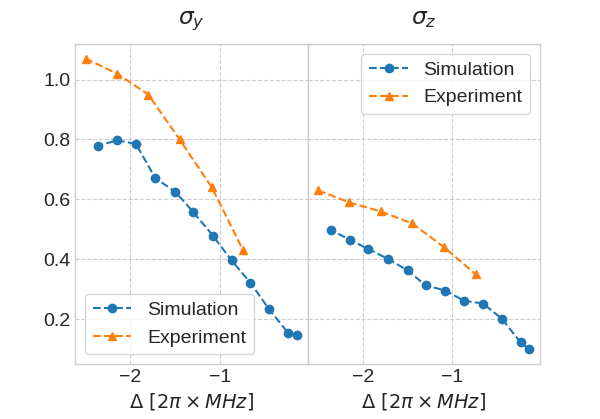
\includegraphics[width=0.6\textwidth]{USPSC-img/dy_cloud_size.png}
    \vspace{5px}
    \legend{Components $ y $ and $ z $ of the cloud size as a function of the laser detuning. The blue spheres and orange triangles are the simulated and experimental cloud sizes respectively.\\ Source: author}
    \label{fig:Dreon-cloud-size}
\end{figure}

\begin{figure}[!ht]
    \centering
    \caption{Cloud size ratio $ \sigma_y / \sigma_z $ and $ \sigma_x $ of the Dreon nMOT}
    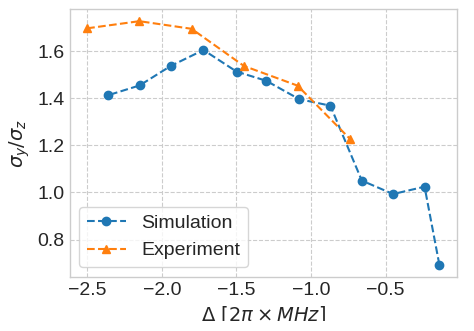
\includegraphics[width=0.55\textwidth]{USPSC-img/dy_cloud_size_ratio.png}
    \vspace{5px}
    \legend{Cloud size ratio $ \sigma_y / \sigma_z $ as a function of the laser detuning. The blue spheres and orange triangles are the simulated and experimental cloud sizes respectively.\\ Source: author}
    \label{fig:Dreon-cloud-size-ratio}
\end{figure}

%-----------------------------------
\subsection{Temperature}
\label{temperature}
%-----------------------------------

The experimental and simulated temperatures are shown in Figure \ref{fig:Dreon-temperature}. Firstly, both simulated and experimental temperatures are higher than the Doppler cooling limit given by $ T_D = 3.26\ \mu K $. For laser detunings roughly larger than $ 6 \Gamma' \simeq 7.5 \Gamma $ in module, the experimental measures match the simulated values. In this range, the temperature is approximately constant, which agrees with the theoretical temperature given by equation (\ref{eq:Doppler-temperature-high-saturation}). However, the absolute theoretical value does not match the experimental measures. For detunings roughly lower than $ 6 \Gamma' $, there is a large divergence between experimental and simulated values. In this range, the nMOT is not in the power-broadened regime.

\begin{figure}[!ht]
    \centering
    \caption{Temperature of the Dreon nMOT as a function of the laser detuning}
    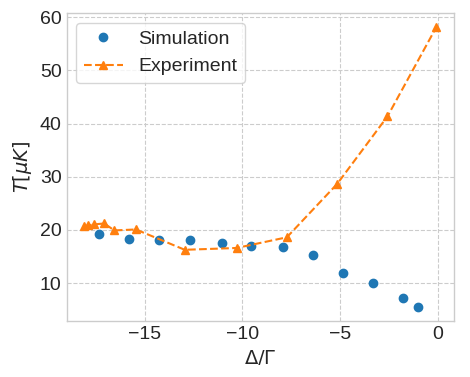
\includegraphics[width=0.55\textwidth]{USPSC-img/dy_temperature.png}
    \vspace{5px}
    \legend{The blue spheres and the orange triangles are the simulated and experimental temperatures respectively. We can roughly split the temperatures into two regions at the laser detuning $ -6 \Gamma' \simeq 7.5 \Gamma $. For detunings lower than $ 6 \Gamma'  $ in module, the nMOT is not in the power-broadened regime and then present a divergence between experimental and simulated values. \\ Source: author}
    \label{fig:Dreon-temperature}
\end{figure}
